\vspace*{-0.05in}
\section{Discussion}
\vspace*{-0.05in}

Long-standing probabilistic models such as copulas \citep{elidan:2013:copulas} and Gaussianization \citep{chen:2000:gaussianization}
can simply represent complex marginal distributions that would require many layers of
transformations in flow-based models like RealNVP and Glow.
Differentiable spline-based coupling layers allow these flows, which are
powerful ways to represent high-dimensional dependencies, to model distributions
with complex shapes more quickly. Our results show that when we have enough
data, the extra flexibility of spline-based layers leads to better
generalization.

For tabular density estimation, both RQ-NSF (C) and RQ-NSF (AR) excel on Power, Gas, and Hepmass, the datasets with the highest ratio of data points to dimensionality from the five considered. 
In image experiments, RQ-NSF (C) achieves the best results on the ImageNet dataset, which has over an order of magnitude more data points than CIFAR-10.
When the dimension is increased without a corresponding increase in dataset size, RQ-NSF still performs competitively with other approaches, but does not outperform them.

\begin{table*}[t!]
	\caption{Test-set bits per dimension (BPD, lower is better) and parameter count for CIFAR-10 and ImageNet64 models. Superscript$^\star$ indicates results are taken from the existing literature.}
	\label{tab:img-results}
        \vspace*{-0.1in}
	\begin{center}
		\begin{small}
			\begin{sc}
				\begin{tabular}{lcccccccc}
					\toprule
					& \multicolumn{2}{c}{CIFAR-10 5-bit} & \multicolumn{2}{c}{CIFAR-10 8-bit} & \multicolumn{2}{c}{ImageNet64 5-bit} & 
					\multicolumn{2}{c}{ImageNet64 8-bit}\\
					\cmidrule(lr){2-3} \cmidrule(lr){4-5} \cmidrule(lr){6-7} \cmidrule(lr){8-9}
                    Model & BPD & Params & BPD & Params & BPD & Params & BPD & Params\\ 
                    \midrule
                    Baseline& $1.70$ & \hphantom{0}5.2M & $3.41$ & 11.1M & $1.81$ & \hphantom{0}14.3M & $3.91$ & \hphantom{0}14.3M \\
                    RQ-NSF (C) & $1.70$ & \hphantom{0}5.3M & $3.38$ & 11.8M & $1.77$ & \hphantom{0}15.6M & $3.82$ & \hphantom{0}15.6M \\
                    \midrule
                    Glow$^\star$ & $1.67$ & 44.0M & $3.35$ & 44.0M & $1.76$ & 110.9M & $3.81$ & 110.9M \\
                    \bottomrule
				\end{tabular}
			\end{sc}
		\end{small}
	\end{center}
	\vspace{-0.5em}
\end{table*}

\newcommand{\fg}{0.45\linewidth}
\begin{figure}[ht]
	\centering
	\begin{tabular}{cc}
		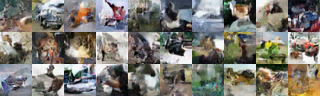
\includegraphics[width=\fg]{figures/images/cifar10-5bit.png} &
		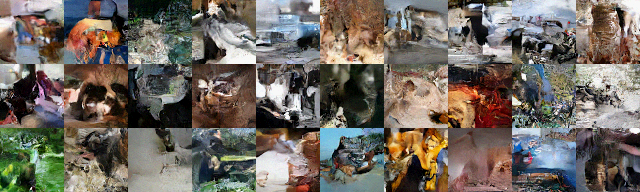
\includegraphics[width=\fg]{figures/images/imagenet64-5bit.png} 
		\\
		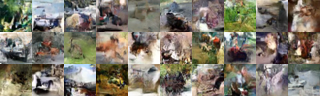
\includegraphics[width=\fg]{figures/images/cifar10-8bit.png} &
		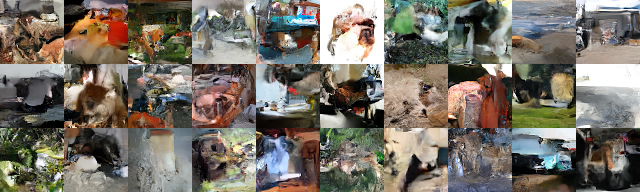
\includegraphics[width=\fg]{figures/images/imagenet64-8bit.png}
	\end{tabular}
        \vspace*{-0.05in}
	\caption{Samples from image models for 5-bit (top) and 8-bit (bottom) datasets. \textbf{Left:} CIFAR-10. \textbf{Right:} ImageNet64.}
	\label{fig:img-samples}
	\vspace{-0.5cm}
\end{figure}

Overall, neural spline flows demonstrate that there is significant performance to be gained by upgrading the commonly-used affine transformations in coupling and autoregressive layers, without the need to sacrifice analytic invertibility. 
Monotonic spline transforms enable models based on coupling layers to achieve density-estimation performance on par with the best autoregressive flows, while retaining exact one-pass sampling. 
These models strike a novel middle ground between flexibility and practicality, providing a useful off-the-shelf tool for the enhancement of architectures like the variational autoencoder, while also improving parameter efficiency in generative modeling.

The proposed transforms scale to high-dimensional problems, as demonstrated empirically.
The only non-constant operation added is the binning of the inputs according to the knot locations, which can be efficiently performed in $\mathcal{O}(\log_{2}K)$ time for $K$ bins with binary search, since the knot locations are sorted.
Moreover, due to the increased flexibility of the spline transforms, we find that we require fewer steps to build flexible flows, reducing the computational cost.
In our experiments, which employ a linear $ \mathcal{O}(K) $ search, we found rational-quadratic splines added approximately 30-40\% to the wall-clock time for a single traning update compared to the same model with affine transformations. 
A potential drawback of the proposed method is a more involved implementation; 
we alleviate this by providing an extensive appendix with technical details, and a reference implementation in PyTorch. 
A third-party implementation has also been added to TensorFlow Probability \citep{dillon2017tensorflowdistributions}.

Rational-quadratic transforms are also a useful differentiable and invertible module in their own right, which could be included in many models that can be trained end-to-end.
For instance, monotonic warping functions with a tractable Jacobian determinant are
useful for supervised learning \citep{snelson:2003:warpedgp}.
More generally, invertibility can be useful for training very large networks, since activations can be recomputed on-the-fly for backpropagation, meaning gradient computation requires memory which is constant instead of linear in the depth of the network \citep{Gomez:2017:revnet, MacKay:2018:revrnn}.
Monotonic splines are one way of constructing invertible elementwise transformations, but there may be others. The benefits of research in this direction are clear, and so we look forward to future work in this area.
